
LVMs are usually applied to the exponential family because inference is feasible in this case. Neural network have recent enabled LVMs to be extended outside the exponential family, for example, \emph{variational auto-encoders} or \emph{VAEs} (\cite{kingma2013auto}) are the most influential models combining both concepts. They extent the classical \emph{principal components analysis} (PCA~\cite{pearson1901liii}) technique for  reduction. Suppose we have a \(D\)-dimensional representation of a data point \(x\) and \(z\) is its latent \(K\)-dimensional representation (\(K < D\)). PCA computes an affine transformation \(\bm{W}\), represented by a \(K \times D\) matrix.

Whereas the PCA reduction is usually computed using either the singular value decomposition or the eigenvalue decomposition of the covariance matrix of the original data, a probabilistic view of PCA can be modeled with an LVM (\cite{tipping1999probabilistic}). The following elements are considered:

\begin{itemize}
  \item \(\bX = \{X_{1},\dots,X_{N}\}\) i.i.d \(\mathbb{R}^{D}\)-valued random variables and the corresponding observations \(\bx = \{x_{1},\dots, x_{N}\}\).
  \item \(\bZ = \{Z_{1}, \dots, Z_{N}\}\) i.i.d latent \(\mathbb{R}^{K}\)-valued random variables, where \(Z_{n}\) models the \(K\)-dimensional representation of \(x_{n}\).
  \item A global latent \(K\times D\)-dimensional random variable \(\bm{W}\), which models the transformation between the spaces.
  \item A noise hyper-parameter \(\sigma^{2}\).
\end{itemize}

\begin{figure}[h!]
  \centering
  \begin{tikzpicture}[
    node distance=1cm and 0.5cm,
    mynode/.style={draw,circle,text width=0.5cm,align=center},
    param/.style={draw,text width=0.5cm,align=center,  fill={rgb:black,1;white,6;blue,0.5}}
    ]

    \node[mynode] (theta) {\(\bm{W}\)};
    \node[mynode, below left=of theta] (zn) {\(Z_{n}\)};
    \node[mynode,  fill={rgb:black,1;white,2}, below right=of theta] (xn) {\(X_{n}\)};
    \node[param, right=of xn] (sigma) {\(\sigma\)};

    \plate[inner sep=.3cm,xshift=.02cm,yshift=.2cm] {} {(zn)(xn)} {\(n = 1\dots N\)}; %
    \path (theta) edge[-latex] (xn)
    (sigma) edge[-latex] (xn)
    (zn) edge[-latex] (xn)
    ;

  \end{tikzpicture}
  \caption{Probabilistic PCA model}\label{fig:ppca}
\end{figure}



We assume the priors are normally distributed:
\[
  Z_{n} \sim \mathcal{N}_{K}(0, I) \quad \forall n =1,\dots,N \quad \text{ and } \quad \bm{W} \sim \mathcal{N}_{K\times D}(0, I).
\]
The data points are considered to be generated via a projection to the higher dimensional space,
\[
  X_{n} \mid z_{n}, \bm{w} \sim \mathcal{N}_{D}(\bm{w}^{T}z_{n}, \sigma^{2}I)\quad \forall n = 1,\dots, N.
\]
The probabilistic model extends the classical one in the way that the latter assumes the noise is infinitesimally small, i.e, \(\sigma^{2} \to 0\). The \emph{expectation-maximization algorithm} (Chapter~\ref{ch:vi_em}) is commonly used to solve this variational inference problem.

There exists other approaches for the PCA model, for example, another variable \(\delta\) might be considered in order to produce non-centered points, that is,
\[
  \delta \sim \mathcal{N}_{D}(0, I) \quad \text{and} \quad   X_{n} \mid z_{n}, \bm{w}, \delta \sim \mathcal{N}(\bm{w}^{T}z_{n} + \delta, \sigma^{2}I)\quad \forall n = 1,\dots, N.
\]

\section{Artificial neural networks}

An \emph{artificial neural network} or \emph{ANN} with \(L\) hidden layers can be defined as a deterministic non-linear function \(f\) parameterized by a set of matrices \(\bm{W} = \{\bm{W}_{0},\dots, \bm{W}_{L}\}\) and non-linear activation functions \(\{r_{0},\dots, r_{L}\}\). Given an input \(x\) the output \(y\) of the network is calculated has
\[
  h_{0} = r_{0}(\bm{W}^{T}_{0}x), \quad \dots \quad h_{l} = r_{l}(\bm{W}_{l}^{T}h_{l-1}), \quad \dots \quad y = r_{L}(\bm{W}_{L}^{T}h_{L-1}).
\]

\emph{Deep neural networks} or \emph{DNNs} are ANNs where the number of hidden layers is considered high. Commonly, any neural network with more that 2 hidden layers is said deep. Given a dataset (set of inputs and their corresponding outputs) \(\{(x_{1}, y_{1}), \dots, (x_{N}, y_{N})\}\) and a loss function \(l(y,y^{*})\) that defines how well the output \(y^{*} = f_{\bm{W}}(x)\)  returned by the network matches the real output \(y\), learning reduces to the optimization problem
\[
  \bm{W}^{opt} = \argmin_{\bm{W}} \sum_{n=1}^{N}l(y_{n}, f_{\bm{W}}(x_{n})).
\]

This problem is usually solved by applying a variant of the \emph{stochastic gradient descent method} (\cite{kiefer1952stochastic}), which is an \emph{stochastic approximation} (\cite{Robbins2007ASA}) of the \emph{gradient descend} (\cite{cauchy1847methode}) technique. \emph{Gradient descent} involves the computation of the loss function's gradient with respect to the network's parameter. Let \(\bm{W}_{t}\) be the set of parameters in the iteration \(t^{th}\) and \(f\) the loss function, seen as a function of the parameters. Then, the parameter update is defined as
\[
  \bm{W}_{t+1} = \bm{W}_{t} + \gamma \nabla f(\bm{W}_{t}).
\]
Where \(\gamma \in \mathbb{R}^{+}\) is a small value. This technique uses the fact that \(- \nabla f(\bm{W})\) points to the local minima in which neighborhood \(\bm{W}\) is. This iterative method guarantees to converge to a local minima, in case \(f\) is convex, gradient descent converges to the global minima.

As the loss function is typically unknown, the gradient estimated using the given dataset. In comparison, \emph{stochastic gradient descent} computes an approximation of the gradient from a randomly selected subset of the data.

The algorithm for computing this gradient is known as \emph{back-propagation} (\cite{goodfellow2016deep}), which is based on a recursive application of the chain-rule of derivatives. This can be implemented using the computational graph on the network.

The main idea of a computational graph is to express a deterministic function, as is the case of a neural network, using an acyclic directed graph. It is composed of input, output and operation nodes, where model data and parameters are shown as input nodes.

\begin{figure}[H]
  \centering
  \begin{tikzpicture}[
    node distance=0.5cm and 1cm,
    mynode/.style={draw,rectangle,minimum size=1cm,,align=center}
    ]

    \node[mynode] (1) {\(*\)};
    \node[left=of 1] (2) {\(4\)};
    \node[above=of 1] (3) {\(x\)};
    \node[mynode, right=of 1] (4) {\(+\)};
    \node[above=of 4] (5) {\(y\)};
    \node[right=of 4] (6) {\(f\)};

    \path (2) edge[-latex] (1)
    (3) edge[-latex] (1)
    (1) edge[-latex] (4)
    (5) edge[-latex] (4)
    (4) edge[-latex] (6)
    ;

  \end{tikzpicture}
  \caption{Computational graph example of function \(f(x,y) = 4x + y\) }\label{fig:cnn_cg}
\end{figure}

The input nodes are typically tensors (\(n\)-dimensional arrays), therefore, the operations are defined over tensors. The main point of using computational graphs is that they enable \emph{automatic differentiation} (\cite{griewank1989automatic}), a technique for computing all partial derivatives of the function.


\section{Non-linear PCA}

\textit{Non-linear PCA} or NLPCA, extends the classical PCA where the relation between the low dimensional space and the observed data is governed by a DNN instead of a linear transformation.
It can be seen as a non-linear probabilistic PCA model.

\begin{figure}[h!]
  \centering
  \begin{tikzpicture}[
    node distance=1cm and 0.5cm,
    mynode/.style={draw,circle,text width=0.5cm,align=center},
    param/.style={draw,text width=0.7cm,align=center, fill={rgb:black,1;white,6;blue,0.5}}
    ]

    \node[mynode] (zn) {\(Z_{n}\)};
    \node[mynode, fill={rgb:black,1;white,2}, right=1.2cm of zn] (xn) {\(X_{n}\)};
    \node[param, above left=of xn] (w0) {\(\bm{W}_0\)};
    \node[param, above right = of xn] (w1) {\(\bm{W}_1\)};

    \plate [inner sep=.3cm,xshift=.02cm,yshift=.2cm]{} {(zn)(xn)} {\(n = 1\dots N\)}; %
    \path (w0) edge[-latex] (xn)
    (w1) edge[-latex] (xn)
    (zn) edge[-latex] (xn)
    ;

  \end{tikzpicture}
  \caption{Non-linear PCA model. \( \bm{W}_0 \) and \( \bm{W}_1 \)  together with an activation function \(r\) represent an ANN.}\label{fig:ppca}
\end{figure}


The model is quite similar to the one presented for the PCA, the difference comes from the conditional distribution of \(X\), that depends on \(Z\) through a fully-connected ANN with a single hidden layer.

As in the case of the PCA, the prior of the latent variable follows a centered Gaussian
\[
  Z_{n} \sim \mathcal{N}_{K}(0,I) \quad \forall n \in 1,\dots,N.
\]

Let \(D\) be the dimension of the data \(X\) and \(K\) the dimension of the hidden variable \(Z\). Let \(f\) a single hidden layer ANN with input dimension \(Z\) and output dimension \(D\). Where the output is the mean value of the normal distribution under \(X\).

As we are considering a single hidden layer, let \(\bm{W}_{0}\) and \(\bm{W}_{1}\) be the matrices governing that ANN and \(r\) the activation function, the ANN \(f\) is
\[
  f(z_{n}) = \bm{W_{1}}(r(\bm{W}_{0}(z_{n})))),
\]

and the data-points are then generated as
\[
  X_{n}\mid Z_{n} \sim \mathcal{N}_{D}(f(Z_{n}), I) \quad \forall n \in 1,\dots,N.
\]
Where no noise is being considered this time.

\section{Variational auto-encoder (Work in Progress)}

\emph{Variational auto-encoders} or VAEs are a dimensionality reduction model, like PCA and NLPCA.\@ In contrast with this two, this auto-encoders contain two neural networks, one in the \(P\) model (decoder) and another one in the variational model \(Q\) (encoder).

The \(P\) model has the same structure as the non-linear PCA.\@ On the other hand, the  distribution \(Q\) is defined with a reverse ANN, with input dimension \(D\) and output dimension \(K\).

The neural networks can be defined to give an output of double the dimension, that is, the encoder would give a point in with \( 2K \) components, so the first \( K \) are used for the mean and the last \( K \) for the variance of the normal distribution.

In conclusion, the parametric model assumes the data is generated as:
\begin{enumerate}
  \item Get a sample from a standard \(K\)-dimensional Gaussian distribution.
    \[
    Z \sim \mathcal{N}_{K}(0,I).
    \]
  \item The data-point is generated from a Gaussian distribution with mean the image of the neural network on the previous sample. Let \(f\) denote the neural network:
    \[
    X \mid z \sim \mathcal{N}_{D}(f(z), I).
    \]
\end{enumerate}
On the other hand, the variational model supposes the hidden values are generated from the observed ones as:
\begin{enumerate}
  \item Let \(x\) be a sample from a standard Gaussian distribution.
    \[
    X \sim \mathcal{N}_{D}(0,I).
    \]
  \item Let \(g\) denote the neural network from the \(D\) dimensional space to a \(2K\) dimensional one. Let \(\mu\) be the first \(K\) components of \(g(x)\) and \(\sigma\) the last ones.
    \[
    g(x) = (\mu, \sigma).
    \]
  \item The hidden representation of \(x\) is generated as
    \[
    Z \mid x \sim \mathcal{N}_{K}(\mu, \text{\texttt{softplus}}(\sigma)).
    \]
\end{enumerate}

Where, as the standard deviation must have a positive value, we use a \texttt{softplus} function to smoothly approximate a rectifier function (\(\text{ReLU}(x) = \max(x,0)\)), this function is defined as
\[
  \text{\texttt{softplus}}(x) = \log(1 + e^{x}).
\]

\begin{figure}[H]
  \centering
  \begin{tikzpicture}[scale=0.8, transform shape]
    \begin{axis}[every axis plot post/.append style={
        mark=none, domain=-3:5,samples=50,smooth},
      axis x line*=bottom, % no box around the plot, only x and y axis
      axis y line*=left, % the * suppresses the arrow tips
      enlargelimits=lower] % extend the axes a bit to the right and top
      \addplot[black!60!green]{(x>=0)*x};
      \addplot[orange]{ln(1+exp(x))};
    \end{axis}
  \end{tikzpicture}
  \caption{ReLU (green) and softplus (orange) comparison in \([-3, 5]\).}
\end{figure}

Figure~\ref{fig:vae} shows a reduction from a \(6\)-dimensional space to a \(2\)-dimensional space. There, each \(x_{n}\) on the left symbolizes the value on each dimension, \(a_{i}\) symbolize weights of the used neural networks (despite using the same symbols, networks are different) and the activation functions are not represented.

\begin{figure}[h]
  \centering
  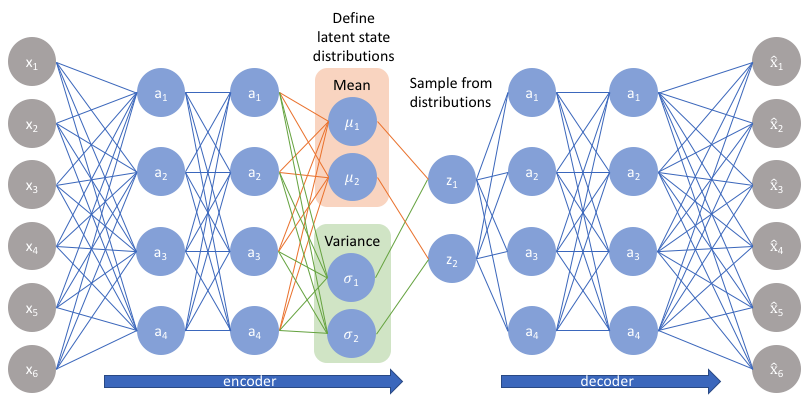
\includegraphics[width=0.8\textwidth]{tex/images/vae.png}
  \caption{Variational auto-encoder structure. Image taken from~\cite{JeremyJordan}.}\label{fig:vae}
\end{figure}
